\chapter{Machine Learning Basics}
In this chapter, we introduce the basics of machine learning. {Deep learning} is a specific kind of machine learning. In order to understand deep learning well, one must have a solid understanding of the basic principles of machine learning.
\section{What is a learning algorithm?}
   	A \textbf{machine learning algorithm} is an algorithm that is able to learn from data. But	what do we mean by learning? Mitchell (1997) provides the definition "A computer program is said to learn from experience $E$	with respect to some class of tasks	$T$	and performance measure	$P$, if its performance at tasks in	$T$, as measured by $P$, improves with experience $E$."

\subsection{The Task, $T$}
Two of most useful examples:
\begin{itemize}
\item \textbf{Classification}: In this type of task, the computer program is asked to specify which of $k$ categories some input belongs to (see \eqref{1}).To solve this task, the learning algorithm is usually asked to produce a function $f:\mathbb R^n \rightarrow \{1,...,k\}$. When $y=f(\bm x)$, the model assigns an input described by vector $\bm x$ to a category identified by numeric code $y$.
\item \textbf{Regression}: In this type of task, the computer program is asked to predict a numerical value given some input(see \eqref{2}). To solve this task, the learning algorithm is asked to output a function $f:\mathbb R^n \rightarrow \mathbb R$.
\end{itemize}
Other examples: {\color{red} LZ: Rewrite into a paragraph?Add some stences to finish this section.}
\begin{itemize}
    \item Transcription
    \item Machine translation
    \item Structured output
    \item Anomaly detection
    \item Synthesis and sampling
    \item Imputation of missing values
    \item Denoising
\end{itemize}
    \begin{figure}
        \caption{Classification}
        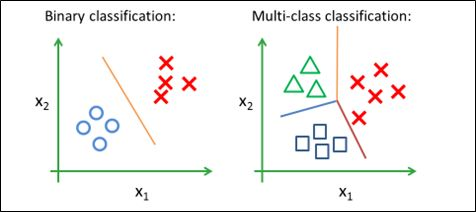
\includegraphics[width=\textwidth]{MachineLearning1}\label{1}
        \caption{Regression}
        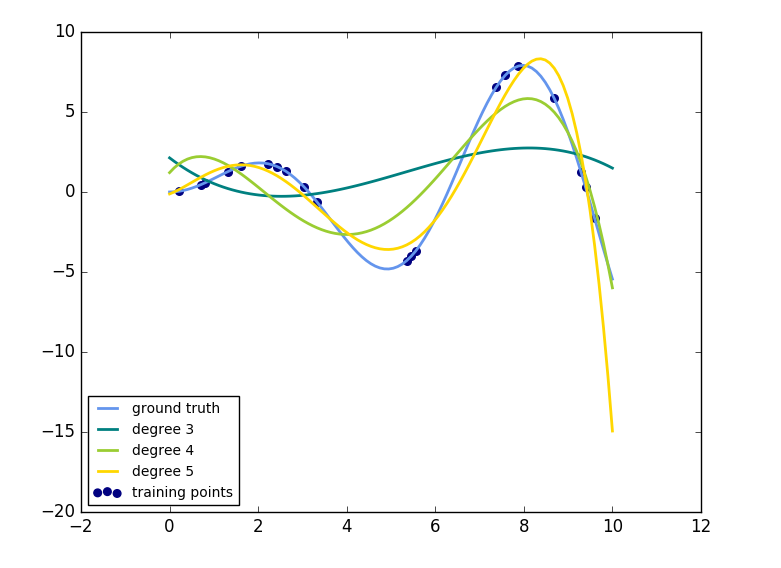
\includegraphics[width=\textwidth]{MachineLearning2}\label{2}
    \end{figure}

\subsection{The Performance Measure, $P$}
\begin{itemize}
    \item In order to evaluate the abilities of a machine learning algorithm, we must design a quantitative measure of its performance. Usually this performance measure $P$ is specific to the task $T$ being carried out by the system.
    
    \item 	Usually we are interested in how well the machine learning algorithm performs	on data that it has not seen before, since this determines how well it will work when deployed in the real world. We therefore evaluate these performance measures using a \textbf{test set} of data that is separate from the data used for training the machine	learning system.
\end{itemize}
\subsection{The Experience, $E$}
        \begin{itemize}
        \item Machine learning algorithms can be broadly categorized as \textbf{unsupervised} or \textbf{supervised}	by what kind of experience they are allowed to have during the learning process. 
        
        \item Traditionally, people refer to regression, classification and structured output problems as supervised learning. Density estimation in
        support of other tasks is usually considered unsupervised learning.
        
        \item Supervised learning examples: Support Vector Machines, Logistic Regression, Decision Tree,...
        \item Unsupervised learning examples: $k$-means Clustering, Principal Components Analysis,...
    \end{itemize}
\subsection{Building a Machine Learning Algorithm}
	
Nearly all deep learning algorithms can be described as particular instances of a fairly simple recipe: combine a specification of a dataset, a cost function, an optimization procedure and a model.

Recognizing that most machine learning algorithms can be described using this recipe helps to see the different algorithms as part of a taxonomy of methods for doing related tasks that work for similar reasons, rather than as a long list of algorithms that each have separate justifications.

For simplicity, we only discuss this kind of machine learning question:
\begin{itemize}
\item $\mathbb X = \{(\bm x^{(1)},y^{(1)}),...,(\bm x^{(m)},y^{(m)})\} \subset \mathbb R^n \times \mathbb R$ is a dataset. Let $\bm X =(\bm x^{(1)},...,\bm x^{(m)})$, $\bm Y=(y^{(1)},...,y^{(m)})$.
\item Let $f:\mathbb R^n\rightarrow \mathbb R$ is function of $\bm x\in \mathbb R^n$, and has parameter $\bm \theta \in \mathbb R^p$, write as $f(\bm x;\bm \theta)$.
\item $\mathcal L:\mathbb R^{m}\times \mathbb R^{m}\rightarrow \mathbb R$ is a function of two $m$-dimensional vectors, usually has formulation like 
$$
\mathcal L(\bm u,\bm v)=\dfrac 1m\sum_{i=1}^m L(u_i,v_i)
$$
where $L(u,v):\mathbb R \times \mathbb R \rightarrow \mathbb R$ is a function describe the error between $u$ and $v$. $J:\mathbb R^p\rightarrow \mathbb R$ is a function of $\bm \theta$ which describes the complexity of $f$.{\color{red} to LZ smooth this sentence.}
\item Let $\bm F(\bm X;\bm \theta)=(f(\bm x^{(1)};\bm \theta),...,f(\bm x^{(m)};\bm \theta))$. Solve:
$$
\bm \theta_{ML}=\arg \min_{\bm \theta}( \mathcal L(\bm F(\bm X;\bm \theta),\bm Y) + J(\bm \theta))
$$
\end{itemize}

\section{Capacity, Overfitting and Underfitting}
\subsection{Generalization}
\begin{itemize}
    \item The central challenge in machine learning is that we must perform well on new, previously unseen inputs---not just those on which our model was trained. The ability to perform well on previously unobserved inputs is called \textbf{generalization}.
    \item Typically, when training a machine learning model, we have access to a training	set, we can compute some error measure on the training set called the \textbf{training	error}, and we reduce this training error.
    \item The \textbf{generalization error}, also called the \textbf{test error} is defined as the expected value of the error on a new input.
    \item We typically estimate the generalization error of a machine learning model by measuring its performance on a \textbf{test set} of examples that were collected separately from the training set.
    
\end{itemize}


\subsection{Data generating distribution}
\marginpar{Wenrui: test}
\begin{itemize}
    \item If the training and the test set are collected arbitrarily, there is indeed little we can
    do. If we are allowed to make some assumptions about how the training and test set are collected, then we can make some progress.
    \item The train and test data are generated by a probability distribution over datasets called the \textbf{data generating process}. We typically make a set of assumptions known collectively as the \textbf{i.i.d. assumptions}{\color{red} LZ: ???}. These assumptions are that the examples in each dataset are	independent from each other, and that the train set and test set are \textbf{identically distributed}, drawn from the same probability distribution as each other. This assumption allows us to describe the data generating process with a probability distribution over a single example. The same distribution is then used to generate every train example and every test example.
    We call that shared underlying distribution the
    data generating distribution, denoted $p_{data}$. 
\end{itemize}
\subsection{Capacity, Underfitting and Overfitting}
\begin{itemize}
    \item How well a machine learning algorithm will perform are its ability to:\\ 1. Make the training error small.\\ 2. Make the gap between training and test error small.
    
    \item These two factors correspond to the two central challenges in machine learning: \textbf{underfitting} and \textbf{overfitting}. Underfitting occurs when the model is not able to obtain a sufficiently low error value on the training set. Overfitting occurs when the gap between the training error and test error is too large. (\eqref{3})
    \item  A model's \textbf {capacity} is its ability to fit a wide variety of functions. We can control whether a model is more likely to overfit or underfit by altering its capacity.
\end{itemize}
\begin{figure}
    \caption{This figure show the relationship between capacity, training error and generalization error}
    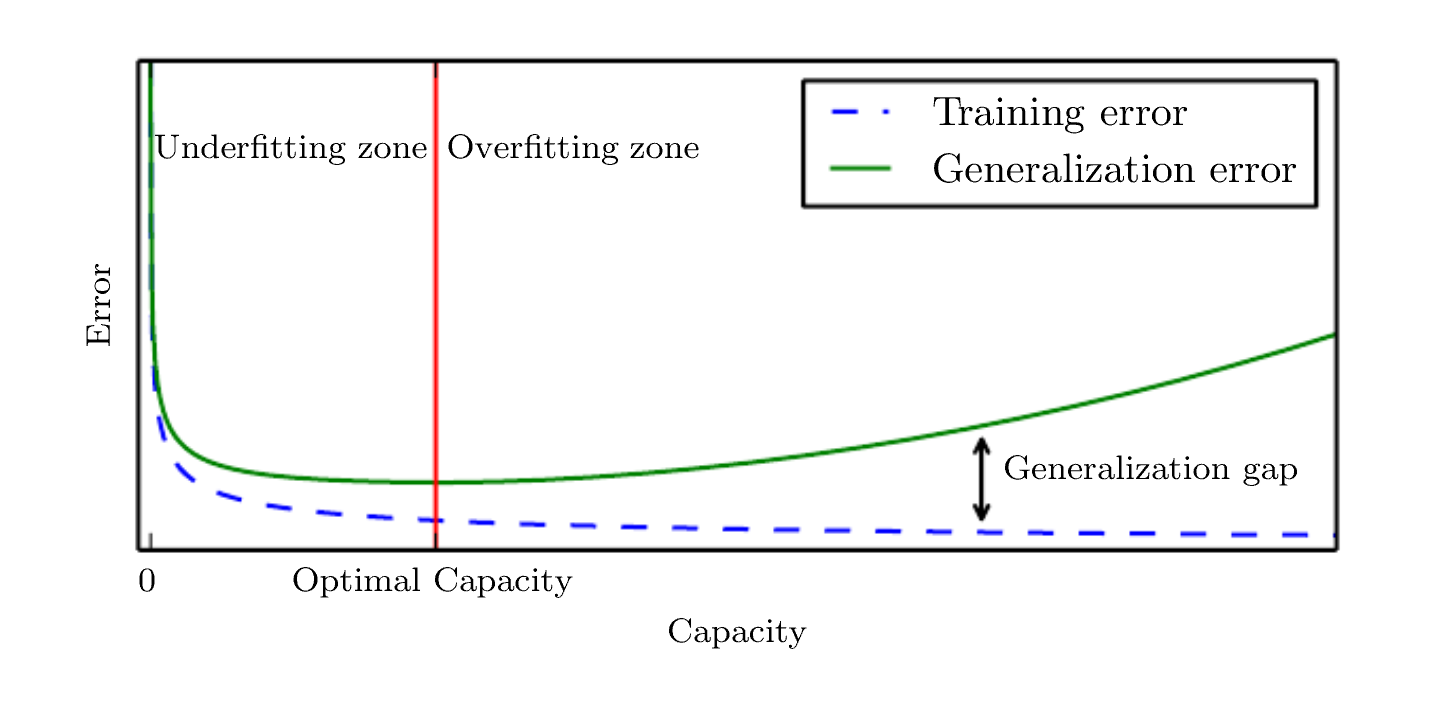
\includegraphics[width=\textwidth]{MachineLearning3}\label{3}
\end{figure}
\subsection{The No Free Lunch Theorem}
    \begin{itemize}
        \item  \textbf{The No Free Lunch Theorem}: Averaged over all possible data generating distributions, every classification algorithm has the
        same error rate when classifying previously unobserved points. In other words, in some sense, no machine learning algorithm is universally any better than any other.
        \item  These results hold only when we average over \underline{all possible data} generating distributions. If we make assumptions about the kinds of probability distributions we encounter in real-world applications, then we can design learning
        algorithms that perform well on these distributions.
    \end{itemize}

\subsection{Regularization}
    \begin{itemize}
        \item There are many ways of expressing preferences for different solutions, both implicitly and explicitly. Together, these different approaches
        are known as regularization. Regularization is any modification we make to a learning algorithm that is intended to reduce its generalization error but not its training error. Regularization is one of the central concerns of the field of machine learning, rivaled in its importance only by optimization.
        \item The no free lunch theorem has made it clear that there is no best machine learning algorithm, and, in particular, no best form of regularization. Instead	we must choose a form of regularization that is well-suited to the particular task we want to solve.
    \end{itemize}

\section{Some Statistical Concepts}
In this section, we introduce some useful concepts in statistical. Machine learning is also called statistical learning, statistical tools play an important role in the analysis of machine learning algorithm. 
\subsection{Estimators}
    \begin{itemize}
        \item The field of statistics gives us many tools that can be used to achieve the machine	learning goal of solving a task not only on the training set but also to generalize.	Foundational concepts such as parameter estimation, bias and variance are useful	to formally characterize notions of generalization, underfitting and overfitting.
        \item Let $\{\mathbf{x}^{(1)},...,\mathbf{x}^{(m)}\}$ be a set of $m$ i.i.d. data points. A \textbf{point estimator} or \textbf{statistic} is any function of the data:
        $$
        \hat{\bm \theta}_m=g(\mathbf{x}^{(1)},...,\mathbf{x}^{(m)}).
        $$
    \end{itemize}


\subsection{Bias and Variance}
    The bias of an estimator is defined as:
    $$
    \text{bias}(\hat{\bm \theta}_m)=\mathbb{E}(\hat{\bm \theta}_m)-\bm \theta
    $$
    where the expectation is over the data (seen as samples from a random variable) and $\bm\theta$ is the true underlying value of $\bm\theta$	used to define the data generating distribution.
    \begin{itemize}
        \item An estimator $\hat{\bm \theta}_m$ is said to be \textbf{unbiased} if bias$(\hat{\bm \theta}_m)=0$,
        which implies that $\mathbb{E}(\hat{\bm \theta}_m)=\bm\theta$.
        \item An estimator $\hat{\bm \theta}_m$ is said to be \textbf{asymptotically unbiased} if $\text{bias}\lim_{m\rightarrow\infty}(\hat{\bm \theta}_m)=0$,
        which implies that $\text{bias}\lim_{m\rightarrow\infty}\mathbb{E}(\hat{\bm \theta}_m)=\bm\theta$.
    \end{itemize}
    The \textbf{Variance} of an estimator is simply the variance $\text{Var} (\hat{\bm \theta}_m)$, where the random variable is the training set.
    

    \begin{itemize}
        \item Bias and variance measure two different sources of error in an estimator. Bias measures the expected deviation from the true value of the function or parameter. Variance on the other hand, provides a measure of the deviation from the expected estimator value that any particular sampling of the data is likely to cause. (\eqref{4})
        \item For \textbf{mean squared error(MSE)}
        $$
        \text{MSE}=\mathbb E[(\hat{\bm \theta}_m-\bm{\theta})]^2=\text{Bias}(\hat{\bm \theta}_m)^2+\text{Var}(\hat{\bm \theta}_m).
        $$
    \end{itemize}

    \begin{figure}
        \caption{ This relationship is similar to the relationship between capacity, underfitting, and overfitting.}
        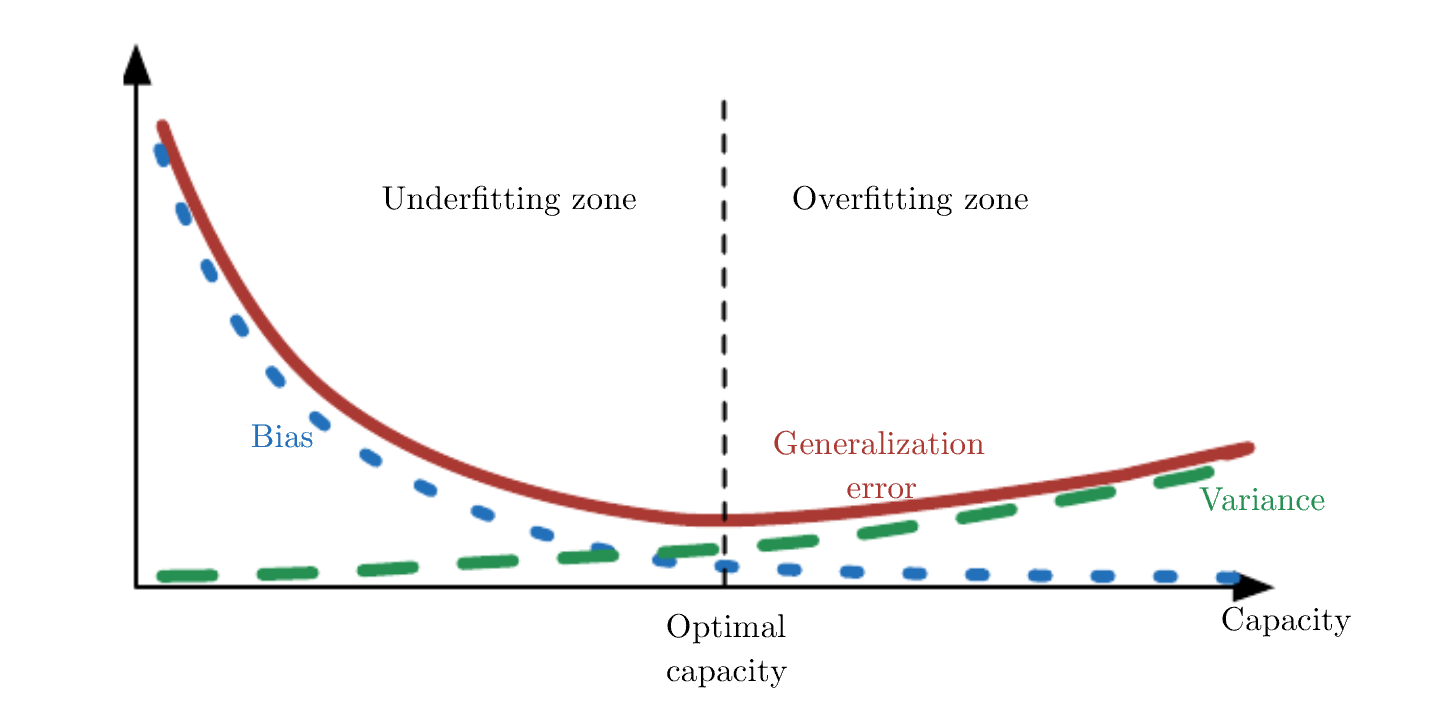
\includegraphics[width=\textwidth]{MachineLearning4}\label{4}
    \end{figure}
\subsection{Maximum Likelihood Estimation}
    \begin{itemize}
        \item Consider a set of $m$ examples $\mathbb X=\{\bm x^{(1)},...,\bm x^{(m)}\}$ drawn independently from the true but unknown data generating distribution $p_{data}(\bm x)$.
        \item Let $p_{model}(\bm x;\bm \theta)$ be a parametric family of probability distributions over the same space indexed by $\bm \theta$.
        \item The maximum likelihood estimator for $\bm \theta$ is then defined as 
        \begin{equation*}
        \begin{split}
        \bm \theta_{ML} &= \arg \max_{\bm \theta}p_{model}(\mathbb X;\bm \theta) \\
        &=\arg \max_{\bm \theta}\prod_{\bm x \in \mathbb X} p_{model}(\bm x;\bm \theta)\\
        &=\arg \max_{\bm \theta}\sum_{\bm x \in \mathbb X} \log p_{model}(\bm x;\bm \theta)\\
        &=\arg \max_{\bm \theta}\mathbb E_{\bm x \sim \hat{p}_{data}} \log p_{model}(\bm x;\bm \theta)
        \end{split}
        \end{equation*}
        where the empirical distribution $\hat{p}_{data}$ defined by the training data.
    \end{itemize}

\subsection{Conditional Log-Likelihood}
    \begin{itemize}
        \item The maximum likelihood estimator can readily be generalized to the case where our goal is to estimate a conditional probability $P(y |\bm x;\bm \theta)$ in order to predict $y$ given $\bm x$. This is actually the most common situation because it forms the basis for most supervised learning. If $\bm X$ represents all our inputs and $\bm Y$	all our observed targets, then the conditional maximum likelihood estimator is
        $$
        \bm \theta_{ML} =\arg\max_{\bm \theta}P(\bm Y|\bm X;\bm \theta).
        $$
        \item If the example are assumed to be i.i.d., then this{\color{red} LZ: log-likelihood} can be decomposed into
        $$
        \bm \theta_{ML} =\arg\max_{\bm \theta}\sum_{i=1}^{m}\log P(y^{(i)}|\bm x^{(i)};\bm \theta).
        $$
    \end{itemize}

\section{Stochastic Gradient Descent}

    Nearly all of deep learning is powered by one very important algorithm: \textbf{stochastic gradient descent} or SGD. Stochastic gradient descent is an extension of the	gradient descent algorithm.
    
    A recurring problem in machine learning is that large training sets are necessary for good generalization, but large training sets are also more computationally expensive.
    
    The cost function used by a machine learning algorithm often decomposes as a	sum over training examples of some per-example loss function.
    
     For example,
        $$
        \mathcal L(\bm\theta)=
        \mathbb E_{\mathbf{x},y \sim \hat{p}_{data}}L(\mathbf{x},y,\bm{\theta})
        =\dfrac1m \sum^m_{i=1}L(\mathbf{x}^{(i)},y^{(i)},\bm{\theta})
        $$
        where L is the per-example loss.
    
    For these additive cost functions, gradient descent requires computing
        $$
        \nabla_{\bm{\theta}}\mathcal L(\bm\theta)=\dfrac1m \sum^m_{i=1}\nabla_{\bm{\theta}}L(\mathbf{x}^{(i)},y^{(i)},\bm{\theta})
        $$
        the  computational cost of this operation is $O(m)$. 
    \textbf{The insight of stochastic gradient descent is that the gradient is an expectation.}   More specifically, 
    $$
    \mathbb E(\nabla f_{i_t}(x))=\nabla f(x)
    $$
    
    The expectation may be approximately estimated using a small set of samples. Specifically, on each step of the algorithm, we can sample a minibatch of examples $\mathbb{B}  = \{ b_1 ,b_2 ,...,b_{m^{'}}\}$ drawn uniformly from the training set.

    The estimate of the gradient is formed as 
        $$
        \mathbf{g} = \dfrac{1}{m^{'}} \sum_{i\in \mathbb{B}} \nabla_{\bm{\theta}}L(\mathbf{x}^{(i)},y^{(i)},\bm{\theta})
        $$
        using examples from the minibatch B.
     The stochastic gradient descent algorithm
        then follows the estimated gradient downhill:
        $$
        \bm \theta \leftarrow \bm \theta -\epsilon \mathbf g
        $$
        where $\epsilon$ is the learning rate.


\subsection{Other Algorithm}
	We briefly list some other algorithm here and we will discuss these algorithm in detail in another chapter. These algorithm are the improvement of SDG and overcome some shortage of SDG and have better performance than SDG in some conditions. {color{red}LZ: SDG->SGD}\\
	
	Let $t\in \mathbb N$, $\bm x_t$ is the point of $t$th step and $\bm g_t$ is the gradient of $t$th step. Besides we define $\Delta \bm x_t=\bm x_{t}-\bm x_{t-1}$ and $\bm g(\bm x)$ is the stochastic gradient descent at point $\bm x$.
    \subsection{Momentum}
    Momentum is a method with some physical background. It has formulation as
    $$
    	\Delta \bm x_t = \rho \Delta \bm x_{t-1} - \epsilon \bm g_{t-1}
    $$
    where the momentum term $\rho$ is set to $0.9$ or a similar value.
    \subsection{Nesterov Momentum}
    %\mgnote{Jinchao}{Yuyan, please add some explanations/definisions for g??gx??}
    Nesterov Momentum is a variant of the momentum method. It's formultion is
    $$
    \Delta \bm x_t = \rho \Delta \bm x_{t-1} -\epsilon \bm g (\bm x_{t-1} + \rho \Delta \bm x_{t-1})
    $$
    where the $\rho$ is almost the same to the momentum method.
    \subsection{Adagrad}
    This algorithm try to adapt the learning rate $\epsilon$ to the parameters. Here is it's formulation:
    $$
    \Delta \bm x_t = \dfrac{ -\epsilon \bm g_{t-1}}{\sqrt{\sum_{\tau =1}^{t-1} |\bm g_{\tau}|^2 + \delta}}
    $$
    \subsection{Adadelta}
    It's an extension of Adagrad and has formulation like
    $$
    \bm n_t = v\bm n_{t-1}+(1-v)|\bm g_{t-1}|^2
    $$
    $$
    \Delta \bm x_t = \dfrac{ -\epsilon \bm g_{t-1}}{\sqrt{\bm  n_t + \delta}}
    $$
    
    
    \begin{figure}
        \caption{The performance of these algorithm}
        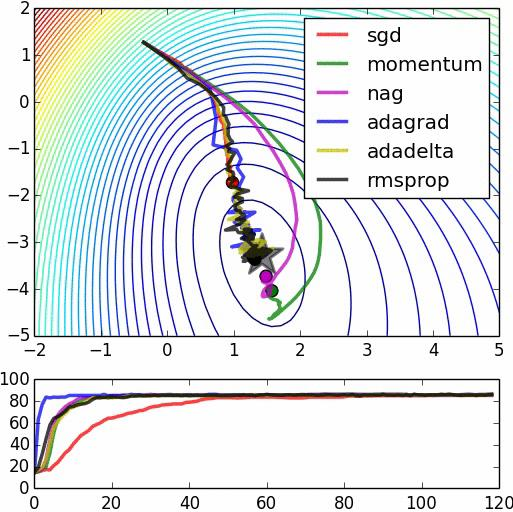
\includegraphics[width= \textwidth]{MachineLearning5}\label{5}
    \end{figure}

\section{Challenges Motivating Deep Learning}


\subsection{Challenges Motivating Deep Learning}
    The simple machine learning algorithms{\color{red}LZ:??} work very well on a wide variety of important problems. However, they have not succeeded in solving the central problems in AI, such as recognizing speech or recognizing objects. The development of deep learning was motivated in part by the failure of traditional algorithms to generalize well on such AI tasks.
    
    Now, let's discuss about how the challenge of generalizing to new examples becomes	exponentially more difficult when working with high-dimensional data, and how the mechanisms used to achieve generalization in traditional machine learning are insufficient to learn complicated functions in high-dimensional spaces. Such spaces also often impose high computational costs. Deep learning was designed to overcome these and other obstacles.


\subsection{The Curse of Dimensionality}
    \begin{itemize}
        \item Many machine learning problems become exceedingly difficult when the number of dimensions in the data is high. This phenomenon is known as the
        \textbf{curse of dimensionality}. The curse of dimensionality arises in many places in computer science, and especially so in machine learning.
        \item One challenge posed by the curse of dimensionality is a statistical challenge. The amount of examples grow quickly while the dimension increases, so a typical grid cell may have no training example associated with it. (\eqref{6})
    \end{itemize}
    \begin{figure}
        \caption{The amount of examples grow quickly while the dimension increases.}
        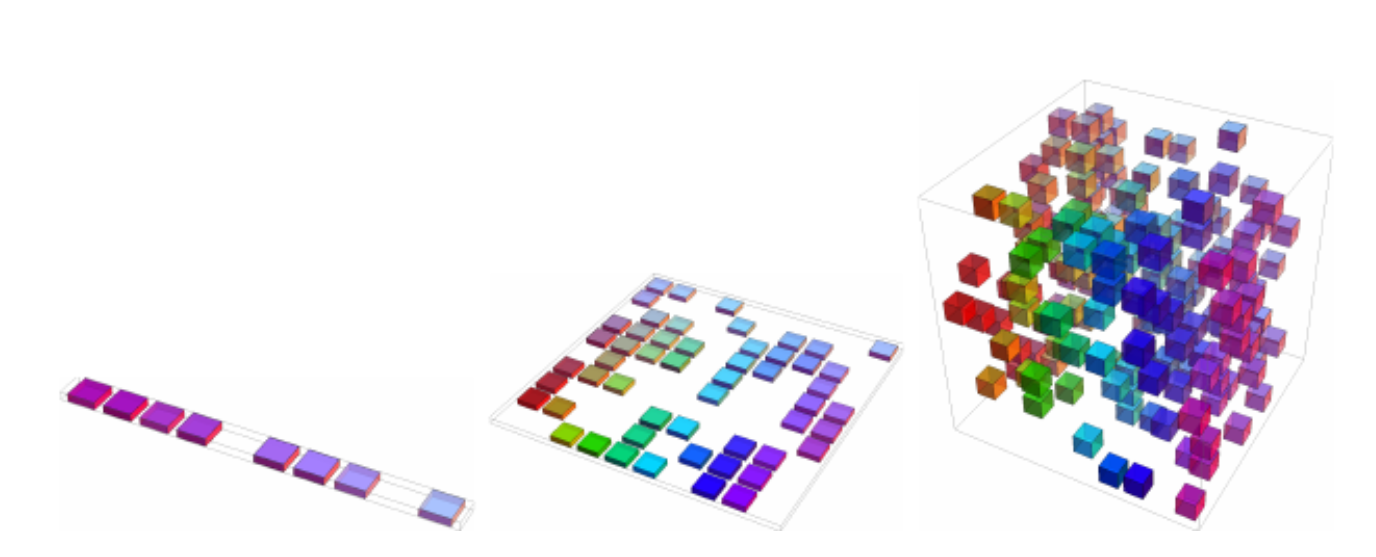
\includegraphics[width = \textwidth]{MachineLearning6}\label{6}
    \end{figure}

    
\subsection{Local Constancy and Smoothness Regularization}
    \begin{itemize}
        \item In order to generalize well, machine learning algorithms need to be guided by prior beliefs about what kind of function they should learn.
        \item Among the most widely used of these implicit ``priors" is the \textbf{smoothness prior} or \textbf{local constancy prior}. This prior states that the function we learn should not change very much within a small region. But AI-level tasks usually do not satisfy this prior.
        \item Many simpler algorithms rely exclusively on this prior to generalize well, and as a result they fail to scale to the statistical challenges involved in solving AI-level tasks.
    \end{itemize}

\subsection{Manifold Learning}
    \begin{itemize}
        \item To put it simply, a \textbf{manifold} is a connected region. Although there is a formal mathematical meaning to the term ``manifold", in
        machine learning it tends to be used more loosely to designate a connected set of points that can be approximated well by considering only a small number of degrees of freedom, or dimensions, embedded in a higher-dimensional space.
        \item Many machine learning problems seem hopeless if we expect the machine learning algorithm to learn functions with interesting variations across all of $\mathbb R^n$.
        \item When the data lies on a low-dimensional manifold, it can be most natural for machine learning algorithms to represent the data in terms of coordinates on the manifold, rather than in terms of coordinates in $\mathbb R^n$.
    \end{itemize}
    \begin{figure} 
    \caption{We'd better regard these data as a 1-D curve than points in $\mathbb R^2$}
    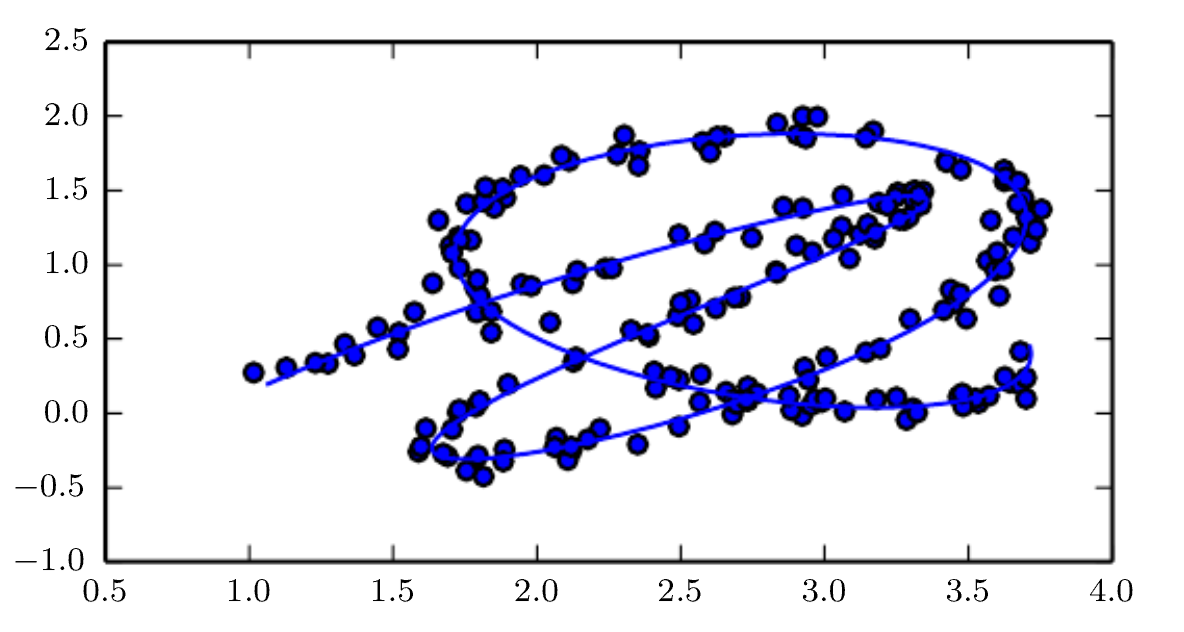
\includegraphics[width =  \textwidth]{MachineLearning7}\label{7}
\end{figure}
